\documentclass[preview]{article}
\usepackage{tikz}
\usepackage{pgfplots}
\usepgfmodule{nonlineartransformations}
\pgfplotsset{compat=1.16}
\pgfkeys{
	/pgfplots/vector plane/.style={
	},
}
\makeatletter
\def\mytransformation{%
	\pgfmathsetmacro{\myX}{\pgf@x}
	\pgfmathsetmacro{\myY}{\pgf@y+0.001*\pgf@x*\pgf@x}
	\setlength{\pgf@x}{\myX pt}
	\setlength{\pgf@y}{\myY pt}
}
\def\testtransform{%
	\pgfmathsetmacro{\myX}{\pgf@x}
	\pgfmathsetmacro{\myY}{\pgf@y+0.00003*\pgf@x*\pgf@x*\pgf@y}
	\setlength{\pgf@x}{\myX pt}
	\setlength{\pgf@y}{\myY pt}
}
\makeatother

\begin{document}
% \begin{figure}
% 	\centering
% 	\begin{tikzpicture}
% 		\begin{scope}
% 			\pgftransformnonlinear{\mytransformation}
% 			\begin{axis}[
% 				width=10cm, height=10cm,
% 				axis x line=middle,
% 				axis y line=middle,
% 				xlabel=$x$,
% 				ylabel=$y$,
% 				every axis x label/.style={
% 					at={(ticklabel* cs:1.02)},
% 					anchor=west,
% 				},
% 				every axis y label/.style={
% 					at={(ticklabel* cs:1.02)},
% 					anchor=south,
% 				},
% 				axis line style={stealth-stealth, thick},
% 				label style={font=\large},
% 				tick label style={font=\large},
% 				xticklabels={,,},
% 				yticklabels={,,},
% 				samples=100,
% 				xmin=-10, xmax=10,
% 				ymin=-10, ymax=10,
% 				grid=both,
% 				major grid style={black!5},
% 				minor grid style={black!5},
% 				]
% 			\end{axis}
% 		\end{scope}
% 	\end{tikzpicture}
% \end{figure}

\vspace{5cm}
\begin{figure}
	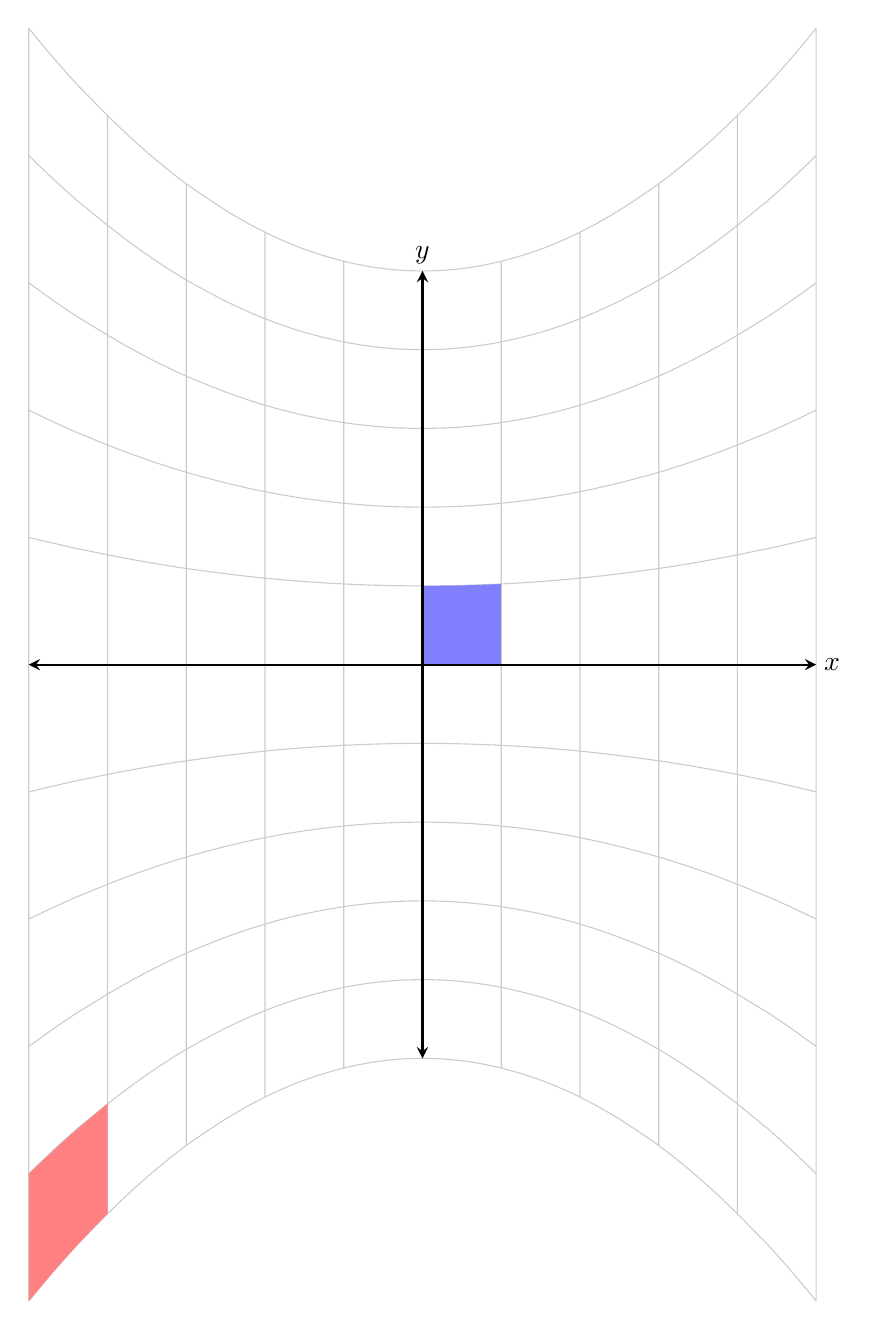
\begin{tikzpicture}
		\begin{scope}
 			\pgftransformnonlinear{\testtransform}
			\draw[step=1, black!20, thin] (-5,-5) grid (5,5);
			\fill[red!50] (-5,-5) rectangle (-4,-4);
			\fill[blue!50] (0,0) rectangle (1,1);
			\draw[stealth-stealth, thick] (-5,0) -- (5,0) node[pos=1.02] {$x$};
			\draw[stealth-stealth, thick] (0,-5) -- (0,5) node[pos=1.02] {$y$};
		\end{scope}
	\end{tikzpicture}
\end{figure}
\end{document}
